\documentclass{elsarticle}

\usepackage[spanish]{babel}
\usepackage{amssymb}
\usepackage{graphicx}
\usepackage{lineno}
\usepackage[utf8]{inputenc}
\usepackage{url}
\usepackage{natbib}
\usepackage{listings}
\usepackage{xcolor}
\usepackage{bera}

\begin{document}
	
\begin{frontmatter}
    \title
    {
        \huge Laboratorio N° 01: \\
        Gestión y planeamiento de pruebas
    }
    \author{Abraham Lipa Calabilla (2019064039)}
    \address{Tacna, Perú}
    \begin{abstract}
        En este documento se describen los pasos para la implementación de un proyecto de ejemplo en Azure DevOps y para el manejo de las pruebas contenidas en el proyecto.
    \end{abstract}
\end{frontmatter}

\section{Titulo}
INFORME DE LABORATORIO N° 01: Gestión y planeamiento de pruebas

\section{Autor}
Abraham Lipa Calabilla

\section{Desarrollo}

\subsection{Preparación de la organización de DevOps}

Nos ubicamos en la organización accediendo a https://dev.azure.com/<organización>/ y hacemos clic en \textbf{Organization settings}.
\begin{center}
	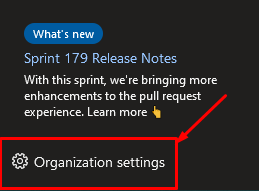
\includegraphics{img/Screenshot_1.png}
\end{center}

En la configuración general, hacemos clic en \textbf{Billing}.
\begin{center}
	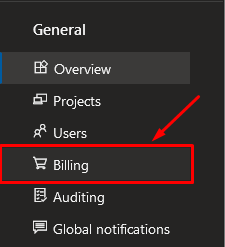
\includegraphics{img/Screenshot_2.png}
\end{center}

Buscamos el sección en la que está \textbf{Basic + Test Plans}. Debe haber un botón para activar la prueba gratuita de \textbf{Test Plans}, hacemos clic, aceptamos y debería salir los días restantes de la prueba.
\begin{center}
	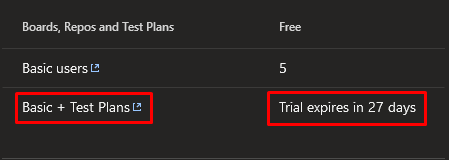
\includegraphics{img/Screenshot_3.png}
\end{center}

Otro apartado necesario es cambiar el nivel de acceso de usuario. Nos ubicamos en la configuración general y hacemos clic en \textbf{Users}.
\begin{center}
	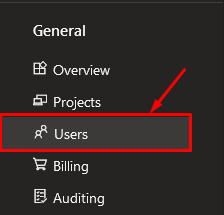
\includegraphics{img/Screenshot_4.png}
\end{center}

En nuestro nombre de usuario, hacemos clic en \textit{más opciones}.
\begin{center}
	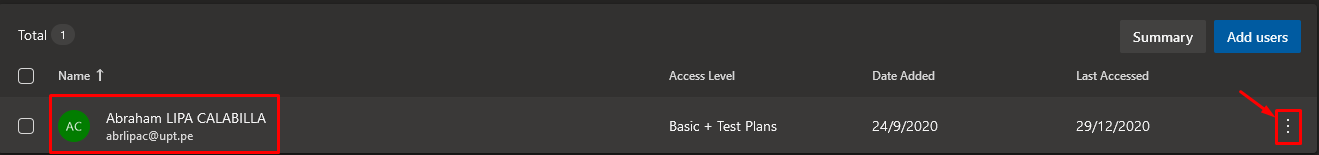
\includegraphics[width=\columnwidth]{img/Screenshot_5.png}
\end{center}

Hacemos clic en \textbf{Change access level}.
\begin{center}
	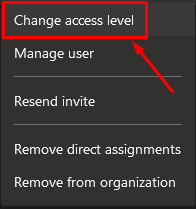
\includegraphics{img/Screenshot_6.png}
\end{center}

En el campo de \textbf{Access level}, cambiamos de \textbf{Basic} a \textbf{Basic + Test Plans}.
\begin{center}
	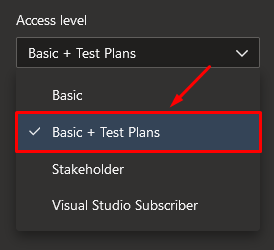
\includegraphics{img/Screenshot_7.png}
\end{center}

Finalmente, guardamos el cambio.
\begin{center}
	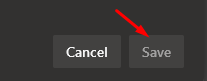
\includegraphics{img/Screenshot_8.png}
\end{center}

\subsection{Configuración del proyecto de ejemplo}

Accedemos a https://azuredevopsdemogenerator.azurewebsites.net/ y, ya en la página, hacemos clic en \textbf{Sign In}.
\begin{center}
	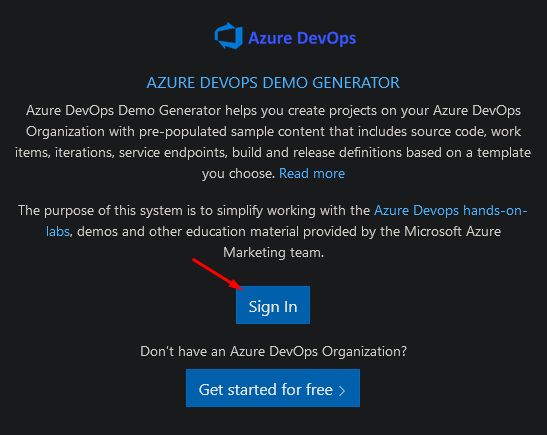
\includegraphics[width=\columnwidth]{img/Screenshot_9.png}
\end{center}

Luego de ingresar las credenciales de nuestra cuenta, en la sección de creación del proyecto:

\begin{enumerate}
    \item Ingresamos un nombre de proyecto
    \item Seleccionamos nuestra organización
    \item Hacemos clic en \textbf{Choose template}
\end{enumerate}

\begin{center}
	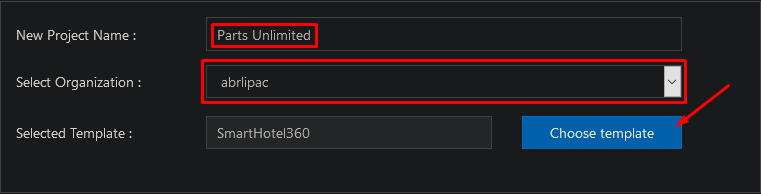
\includegraphics[width=\columnwidth]{img/Screenshot_10.png}
\end{center}

Hacemos clic en \textbf{PartsUnlimited}.
\begin{center}
	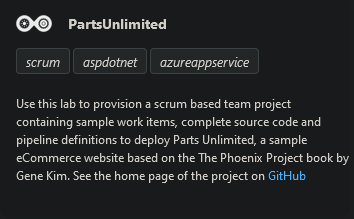
\includegraphics{img/Screenshot_11.png}
\end{center}

Hacemos clic en \textbf{Select Template} para seleccionar la plantilla.
\begin{center}
	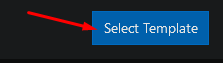
\includegraphics{img/Screenshot_12.png}
\end{center}

Una vez que está seleccionado el proyecto, hacemos clic en \textbf{Create Project}.
\begin{center}
	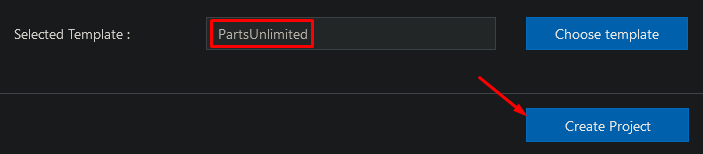
\includegraphics[width=\columnwidth]{img/Screenshot_13.png}
\end{center}

Veremos que el proyecto empieza a crearse.
\begin{center}
	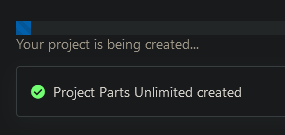
\includegraphics{img/Screenshot_14.png}
\end{center}

Cuando haya terminado el proceso de creación, hacemos clic en \textbf{Navigate to project} para ver el proyecto.
\begin{center}
	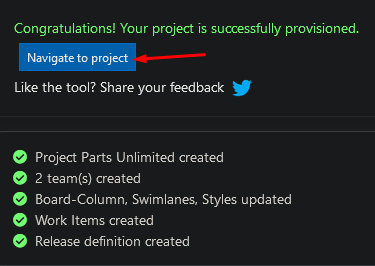
\includegraphics{img/Screenshot_15.png}
\end{center}

Vemos que el proyecto ha sido creado.
\begin{center}
	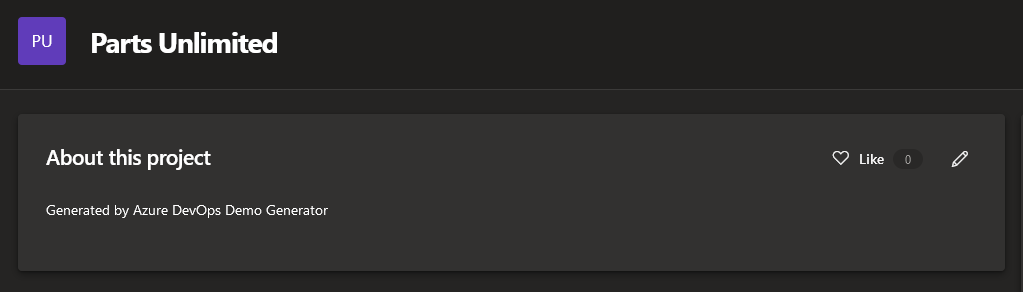
\includegraphics[width=\columnwidth]{img/Screenshot_16.png}
\end{center}

\subsection{Entendiendo los Test Plans, Suites y Cases}

Hacemos clic en Test Plans.
\begin{center}
	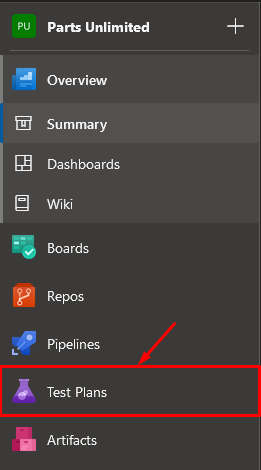
\includegraphics{img/Screenshot_17.png}
\end{center}

Veremos los planes de pruebas, en este caso hay uno llamado \textbf{Parts Unlimited\_TestPlan1}.
\begin{center}
	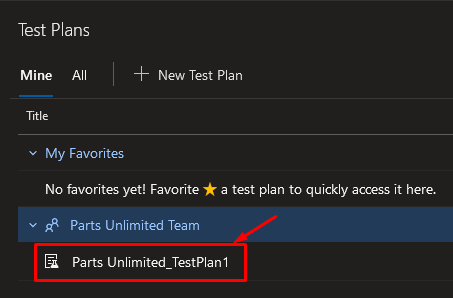
\includegraphics{img/Screenshot_18.png}
\end{center}

Seleccionar la suite de pruebas de la historia \textbf{As a customer, I would like to store my credit card details securely}.
\begin{center}
	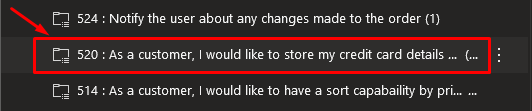
\includegraphics[width=\columnwidth]{img/Screenshot_19.png}
\end{center}

Veremos los casos de prueba de la suite. Luego en la fila del caso de prueba \textbf{Verify that user is allowed to save his credit card detail} hacemos clic \textit{más opciones} y en \textbf{Edit test case}.
\begin{center}
	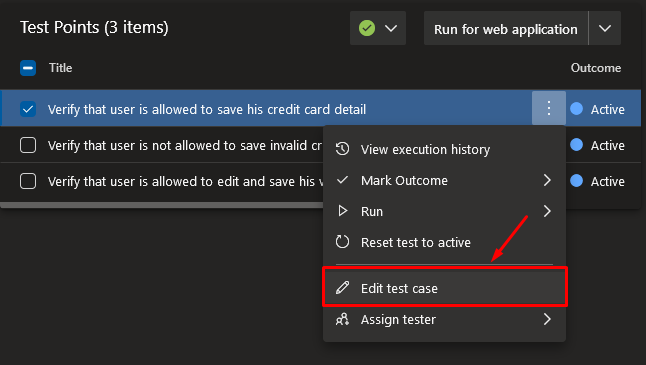
\includegraphics[width=\columnwidth]{img/Screenshot_20.png}
\end{center}

Una vez en los detalles del caso de prueba, hacemos clic en el botón con el icono de \textit{Enlace} para ver los enlaces relacionados al caso de prueba.
\begin{center}
	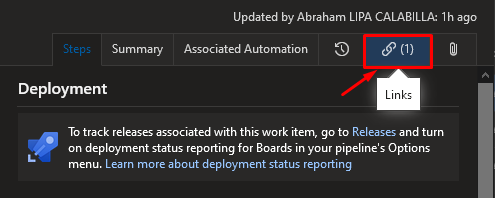
\includegraphics[width=\columnwidth]{img/Screenshot_21.png}
\end{center}

Hacemos clic en \textbf{Add link} y luego en \textbf{Existing item}.
\begin{center}
	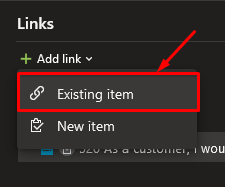
\includegraphics{img/Screenshot_22.png}
\end{center}

Especificamos el tipo de enlace como \textbf{Parent}.
\begin{center}
	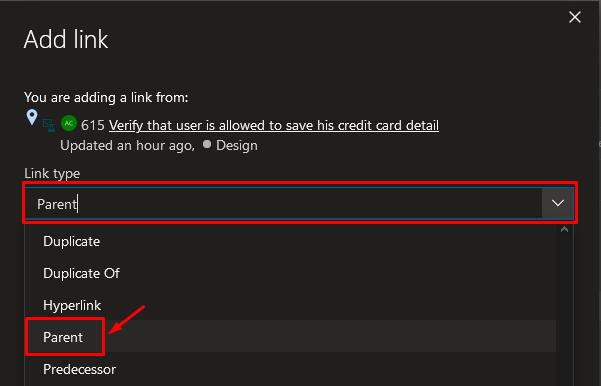
\includegraphics[width=\columnwidth]{img/Screenshot_23.png}
\end{center}

En el campo \textbf{Work items to link}, ingresamos \textit{credit card} y hacemos clic en \textbf{Search} para buscar el \textbf{Work item}.
\begin{center}
	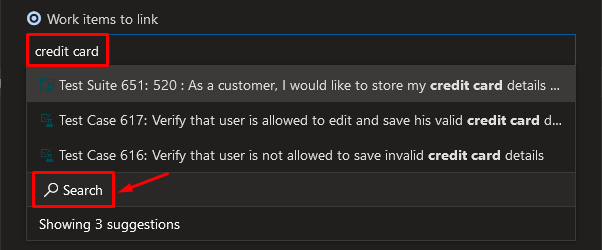
\includegraphics[width=\columnwidth]{img/Screenshot_24.png}
\end{center}

Hacemos clic en el \textbf{Feature Credit Card Purchase}.
\begin{center}
	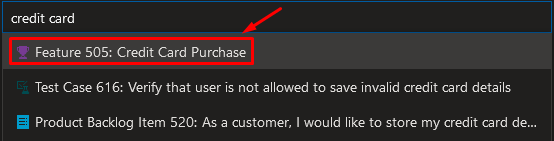
\includegraphics[width=\columnwidth]{img/Screenshot_25.png}
\end{center}

Guardamos el cambio.
\begin{center}
	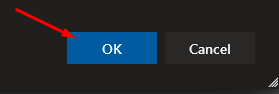
\includegraphics{img/Screenshot_26.png}
\end{center}

Veremos que ahora el caso de prueba está asociado a la característica \textbf{Credit Card Purchase}.
\begin{center}
	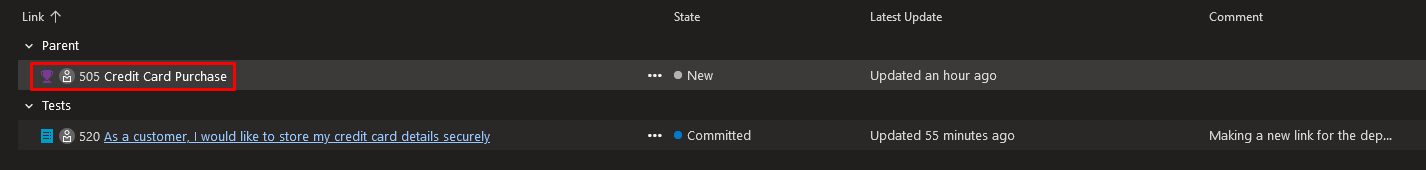
\includegraphics[width=\columnwidth]{img/Screenshot_27.png}
\end{center}

Finalmente, guardamos los cambios y cerramos.
\begin{center}
	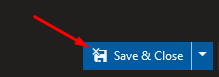
\includegraphics{img/Screenshot_28.png}
\end{center}


\subsection{Manejando las pruebas}

Para cambiar el orden de los casos de prueba de la suite \textbf{As a customer, I would like to store my credit card details securely}, hacemos clic en la suite y luego en la sección \textbf{Define}. En esta sección podemos arrastrar y soltar los casos de pruebas, para luego ver los cmabios reflejados en la propiedad \textbf{Order} de los casos de prueba.
\begin{center}
	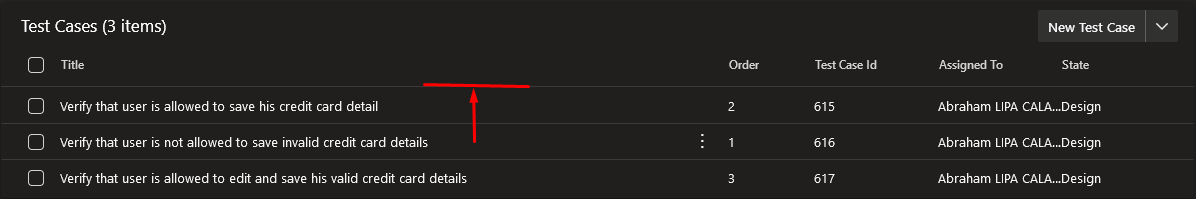
\includegraphics[width=\columnwidth]{img/Screenshot_29.png}
\end{center}

Para cambiar la configuración de los test cases, hacemos clic en \textbf{Configuration}.
\begin{center}
	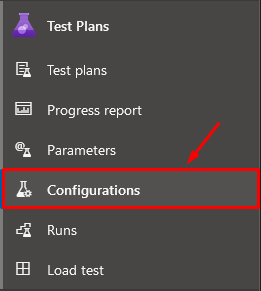
\includegraphics{img/Screenshot_30.png}
\end{center}

Veremos la configuración del sistema operativo \textbf{Windows 10}. Hacemos clic en \textbf{Add configuration variable}.
\begin{center}
	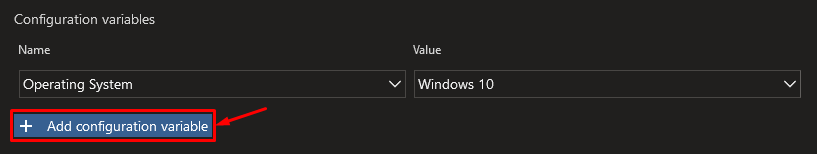
\includegraphics[width=\columnwidth]{img/Screenshot_31.png}
\end{center}

Seleccionamos el nombre \textbf{Browser} y el valor \textbf{Microsoft Edge}.
\begin{center}
	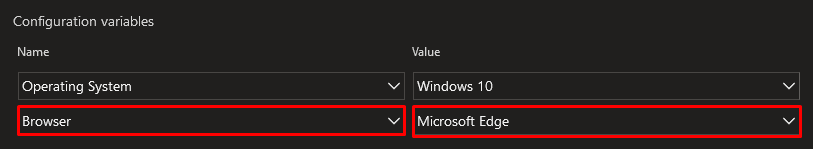
\includegraphics[width=\columnwidth]{img/Screenshot_32.png}
\end{center}

Guardamos el cambio.
\begin{center}
	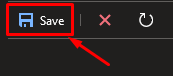
\includegraphics{img/Screenshot_33.png}
\end{center}

Para añadir una nueva configuración para realizar las pruebas en un entorno de \textit{iPhone X}, debemos ubicarnos en la sección \textbf{All configuration variables} hacemos clic en \textbf{Operating System}.
\begin{center}
	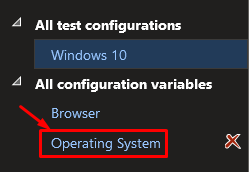
\includegraphics{img/Screenshot_34.png}
\end{center}

Hacemos clic en \textbf{Add new value}.
\begin{center}
	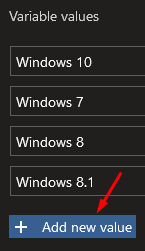
\includegraphics{img/Screenshot_35.png}
\end{center}

Ingresamos el nombre de la configuración \textbf{iOS 12}.
\begin{center}
	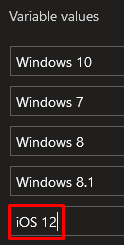
\includegraphics{img/Screenshot_36.png}
\end{center}

Guardamos el cambio.
\begin{center}
	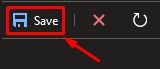
\includegraphics{img/Screenshot_37.png}
\end{center}

Hacemos clic en el botón \textbf{+}.
\begin{center}
	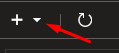
\includegraphics{img/Screenshot_38.png}
\end{center}

Para agregar una nueva configuración de pruebas, hacemos en \textbf{New test configuration}.
\begin{center}
	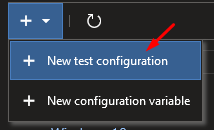
\includegraphics{img/Screenshot_39.png}
\end{center}

En el campo nombre ingresamos \textbf{iPhone 12}. En la sección de las variables de configuración, hacemos clic en \textbf{Add configuration variable} dos veces y seleccionamos el \textbf{Browser} con el valor \textbf{Safari} y el \textbf{Operating System} con el valor \textbf{iOS 12}.
\begin{center}
	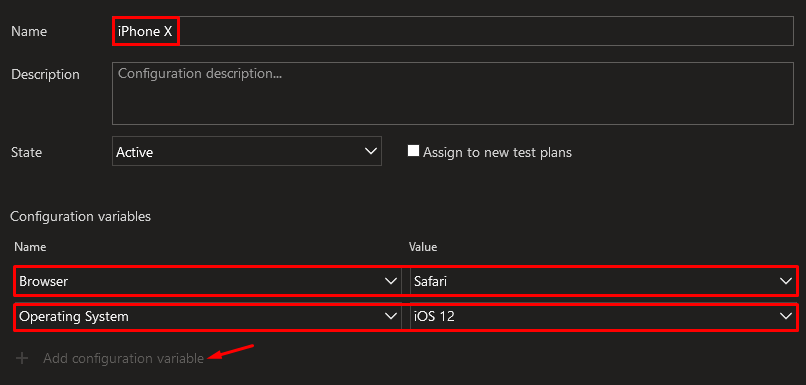
\includegraphics[width=\columnwidth]{img/Screenshot_40.png}
\end{center}

Guardamos el cambio.
\begin{center}
	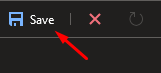
\includegraphics{img/Screenshot_41.png}
\end{center}

Hacemos clic en \textbf{Test plans}.
\begin{center}
	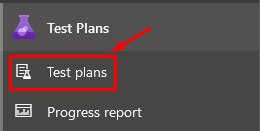
\includegraphics{img/Screenshot_42.png}
\end{center}

En al suite de pruebas \textbf{As a customer, I would like to store my credit card details securely}, hacemos clic derecho y luego clic en \textbf{Assign configurations}.
\begin{center}
	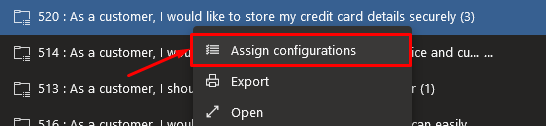
\includegraphics[width=\columnwidth]{img/Screenshot_43.png}
\end{center}

Seleccionamos la configuración de \textbf{iPhone X}.
\begin{center}
	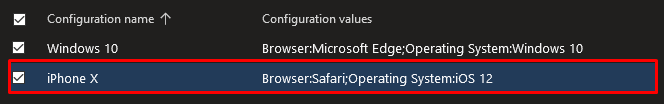
\includegraphics[width=\columnwidth]{img/Screenshot_44.png}
\end{center}

Guardamos el cambio.
\begin{center}
	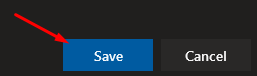
\includegraphics{img/Screenshot_45.png}
\end{center}

En los test cases de la suite podemos ver que se han agregado las pruebas con la configuración del \textbf{iPhone X}.
\begin{center}
	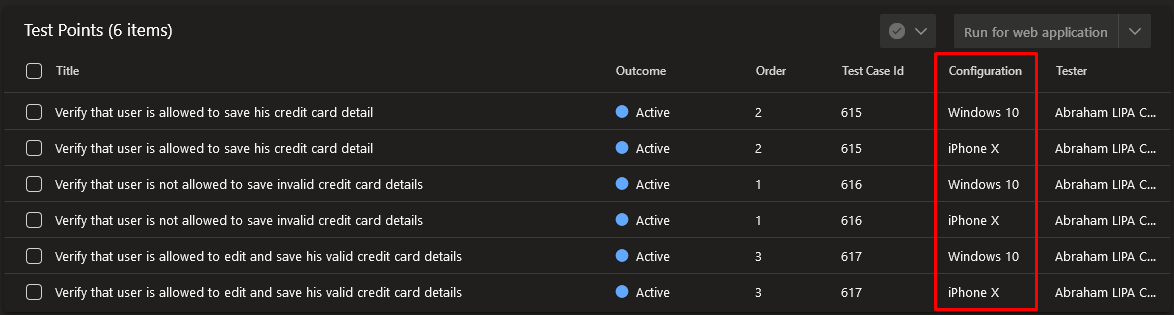
\includegraphics[width=\columnwidth]{img/Screenshot_46.png}
\end{center}

\subsection{Autoría de las pruebas}

En el plan de pruebas, hacemos clic en \textbf{más opciones}, luego en \textbf{New suite} y luego en \textbf{Static suite}.
\begin{center}
	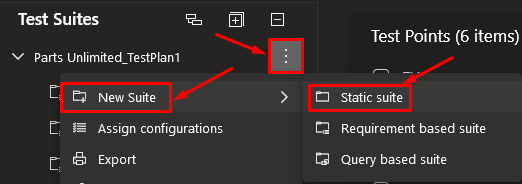
\includegraphics[width=\columnwidth]{img/Screenshot_47.png}
\end{center}

Ingresamos el nombre de la suite como \textbf{Shipping tests}.
\begin{center}
	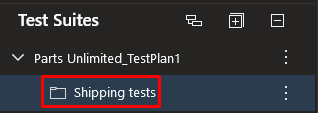
\includegraphics{img/Screenshot_48.png}
\end{center}

En la suite creada, hacemos clic en \textbf{New suite} y luego en \textbf{Requirement based suite}.
\begin{center}
	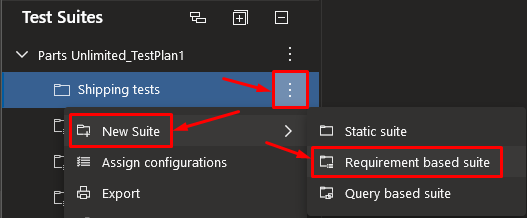
\includegraphics[width=\columnwidth]{img/Screenshot_49.png}
\end{center}

Sin especificar la consulta para devolver los requerimientos, hacemos clic en \textbf{Run query}. Seleccionamos los requerimientos indicados y luego hacemos clic en \textbf{Create suites}.
\begin{center}
	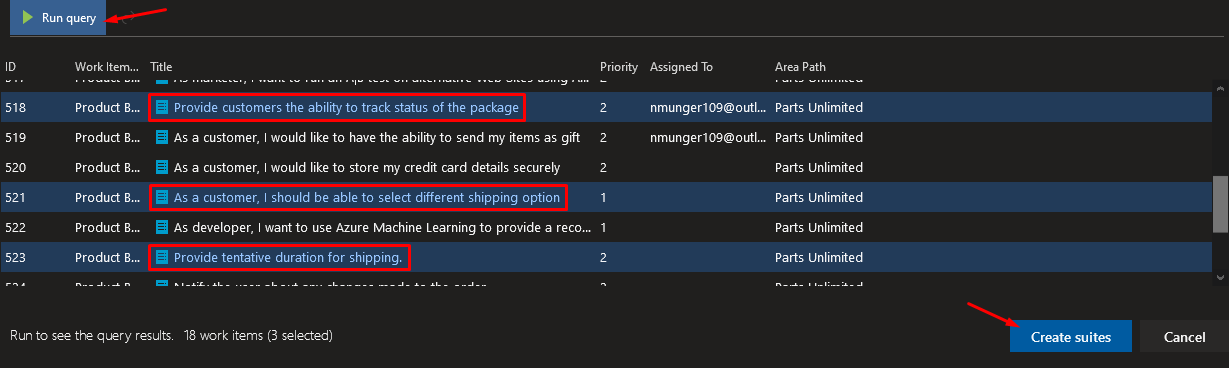
\includegraphics[width=\columnwidth]{img/Screenshot_50.png}
\end{center}

Veremos que se han creado las suites de pruebas en la suite \textbf{Shipping tests} creada previamente.
\begin{center}
	\includegraphics[width=\columnwidth]{img/Screenshot_51.png}
\end{center}

Hacemos clic en la suite \textbf{Provide customers the ability to track status of the package}.
\begin{center}
	\includegraphics[width=\columnwidth]{img/Screenshot_53.png}
\end{center}

Hacemos clic en \textbf{New Test Case} y en \textbf{Add test cases using grid}.
\begin{center}
	\includegraphics{img/Screenshot_52.png}
\end{center}

Agregamos algunos casos de prueba, especificando el título, la acción y el resultado esperado. Luego hacemos clic en \textbf{guardar todo}.
\begin{center}
	\includegraphics[width=\columnwidth]{img/Screenshot_54.png}
\end{center}

Hacemos clic en el botón de vista de grilla.
\begin{center}
	\includegraphics{img/Screenshot_60.png}
\end{center}

Veremos los casos de la siguiente forma:
\begin{center}
	\includegraphics[width=\columnwidth]{img/Screenshot_55.png}
\end{center}

En cambio, si elegimos la vista de lista, los veremos así:
\begin{center}
	\includegraphics{img/Screenshot_56.png}
\end{center}

Otra opción para crear suites es mediante una work item query. En la suite \textbf{Shipping tests}, hacemos clic en \textbf{más opciones}, en \textbf{New suite} y luego en \textbf{Query based suite}.
\begin{center}
	\includegraphics[width=\columnwidth]{img/Screenshot_57.png}
\end{center}

Nos aseguramos que el Work item type sea \textbf{Microsoft.TestCaseCategory} y hacemos clic en \textbf{Run query}.
\begin{center}
	\includegraphics[width=\columnwidth]{img/Screenshot_58.png}
\end{center}

Finalmente veremos la lista de los casos de prueba que podemos agregar.
\begin{center}
	\includegraphics[width=\columnwidth]{img/Screenshot_59.png}
\end{center}

\end{document}
